\documentclass[1p]{elsarticle_modified}
%\bibliographystyle{elsarticle-num}

%\usepackage[colorlinks]{hyperref}
%\usepackage{abbrmath_seonhwa} %\Abb, \Ascr, \Acal ,\Abf, \Afrak
\usepackage{amsfonts}
\usepackage{amssymb}
\usepackage{amsmath}
\usepackage{amsthm}
\usepackage{scalefnt}
\usepackage{amsbsy}
\usepackage{kotex}
\usepackage{caption}
\usepackage{subfig}
\usepackage{color}
\usepackage{graphicx}
\usepackage{xcolor} %% white, black, red, green, blue, cyan, magenta, yellow
\usepackage{float}
\usepackage{setspace}
\usepackage{hyperref}

\usepackage{tikz}
\usetikzlibrary{arrows}

\usepackage{multirow}
\usepackage{array} % fixed length table
\usepackage{hhline}

%%%%%%%%%%%%%%%%%%%%%
\makeatletter
\renewcommand*\env@matrix[1][\arraystretch]{%
	\edef\arraystretch{#1}%
	\hskip -\arraycolsep
	\let\@ifnextchar\new@ifnextchar
	\array{*\c@MaxMatrixCols c}}
\makeatother %https://tex.stackexchange.com/questions/14071/how-can-i-increase-the-line-spacing-in-a-matrix
%%%%%%%%%%%%%%%

\usepackage[normalem]{ulem}

\newcommand{\msout}[1]{\ifmmode\text{\sout{\ensuremath{#1}}}\else\sout{#1}\fi}
%SOURCE: \msout is \stkout macro in https://tex.stackexchange.com/questions/20609/strikeout-in-math-mode

\newcommand{\cancel}[1]{
	\ifmmode
	{\color{red}\msout{#1}}
	\else
	{\color{red}\sout{#1}}
	\fi
}

\newcommand{\add}[1]{
	{\color{blue}\uwave{#1}}
}

\newcommand{\replace}[2]{
	\ifmmode
	{\color{red}\msout{#1}}{\color{blue}\uwave{#2}}
	\else
	{\color{red}\sout{#1}}{\color{blue}\uwave{#2}}
	\fi
}

\newcommand{\Sol}{\mathcal{S}} %segment
\newcommand{\D}{D} %diagram
\newcommand{\A}{\mathcal{A}} %arc


%%%%%%%%%%%%%%%%%%%%%%%%%%%%%5 test

\def\sl{\operatorname{\textup{SL}}(2,\Cbb)}
\def\psl{\operatorname{\textup{PSL}}(2,\Cbb)}
\def\quan{\mkern 1mu \triangleright \mkern 1mu}

\theoremstyle{definition}
\newtheorem{thm}{Theorem}[section]
\newtheorem{prop}[thm]{Proposition}
\newtheorem{lem}[thm]{Lemma}
\newtheorem{ques}[thm]{Question}
\newtheorem{cor}[thm]{Corollary}
\newtheorem{defn}[thm]{Definition}
\newtheorem{exam}[thm]{Example}
\newtheorem{rmk}[thm]{Remark}
\newtheorem{alg}[thm]{Algorithm}

\newcommand{\I}{\sqrt{-1}}
\begin{document}

%\begin{frontmatter}
%
%\title{Boundary parabolic representations of knots up to 8 crossings}
%
%%% Group authors per affiliation:
%\author{Yunhi Cho} 
%\address{Department of Mathematics, University of Seoul, Seoul, Korea}
%\ead{yhcho@uos.ac.kr}
%
%
%\author{Seonhwa Kim} %\fnref{s_kim}}
%\address{Center for Geometry and Physics, Institute for Basic Science, Pohang, 37673, Korea}
%\ead{ryeona17@ibs.re.kr}
%
%\author{Hyuk Kim}
%\address{Department of Mathematical Sciences, Seoul National University, Seoul 08826, Korea}
%\ead{hyukkim@snu.ac.kr}
%
%\author{Seokbeom Yoon}
%\address{Department of Mathematical Sciences, Seoul National University, Seoul, 08826,  Korea}
%\ead{sbyoon15@snu.ac.kr}
%
%\begin{abstract}
%We find all boundary parabolic representation of knots up to 8 crossings.
%
%\end{abstract}
%\begin{keyword}
%    \MSC[2010] 57M25 
%\end{keyword}
%
%\end{frontmatter}

%\linenumbers
%\tableofcontents
%
\newcommand\colored[1]{\textcolor{white}{\rule[-0.35ex]{0.8em}{1.4ex}}\kern-0.8em\color{red} #1}%
%\newcommand\colored[1]{\textcolor{white}{ #1}\kern-2.17ex	\textcolor{white}{ #1}\kern-1.81ex	\textcolor{white}{ #1}\kern-2.15ex\color{red}#1	}

{\Large $\underline{12n_{0416}~(K12n_{0416})}$}

\setlength{\tabcolsep}{10pt}
\renewcommand{\arraystretch}{1.6}
\vspace{1cm}\begin{tabular}{m{100pt}>{\centering\arraybackslash}m{274pt}}
\multirow{5}{120pt}{
	\centering
	\includegraphics[width=112pt]{../../../GIT/diagram.site/Diagrams/png/2505_12n_0416.png}\\
\ \ \ A knot diagram\footnotemark}&
\allowdisplaybreaks
\textbf{Linearized knot diagam} \\
\cline{2-2}
 &
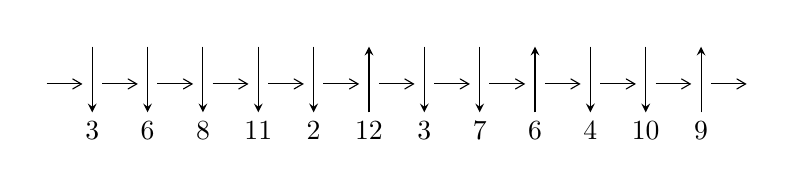
\begin{tikzpicture}[x=20pt, y=17pt]
	% nodes
	\node (C0) at (0, 0) {};
	\node (C1) at (1, 0) {};
	\node (C1U) at (1, +1) {};
	\node (C1D) at (1, -1) {3};

	\node (C2) at (2, 0) {};
	\node (C2U) at (2, +1) {};
	\node (C2D) at (2, -1) {6};

	\node (C3) at (3, 0) {};
	\node (C3U) at (3, +1) {};
	\node (C3D) at (3, -1) {8};

	\node (C4) at (4, 0) {};
	\node (C4U) at (4, +1) {};
	\node (C4D) at (4, -1) {11};

	\node (C5) at (5, 0) {};
	\node (C5U) at (5, +1) {};
	\node (C5D) at (5, -1) {2};

	\node (C6) at (6, 0) {};
	\node (C6U) at (6, +1) {};
	\node (C6D) at (6, -1) {12};

	\node (C7) at (7, 0) {};
	\node (C7U) at (7, +1) {};
	\node (C7D) at (7, -1) {3};

	\node (C8) at (8, 0) {};
	\node (C8U) at (8, +1) {};
	\node (C8D) at (8, -1) {7};

	\node (C9) at (9, 0) {};
	\node (C9U) at (9, +1) {};
	\node (C9D) at (9, -1) {6};

	\node (C10) at (10, 0) {};
	\node (C10U) at (10, +1) {};
	\node (C10D) at (10, -1) {4};

	\node (C11) at (11, 0) {};
	\node (C11U) at (11, +1) {};
	\node (C11D) at (11, -1) {10};

	\node (C12) at (12, 0) {};
	\node (C12U) at (12, +1) {};
	\node (C12D) at (12, -1) {9};
	\node (C13) at (13, 0) {};

	% arrows
	\draw[->,>={angle 60}]
	(C0) edge (C1) (C1) edge (C2) (C2) edge (C3) (C3) edge (C4) (C4) edge (C5) (C5) edge (C6) (C6) edge (C7) (C7) edge (C8) (C8) edge (C9) (C9) edge (C10) (C10) edge (C11) (C11) edge (C12) (C12) edge (C13) ;	\draw[->,>=stealth]
	(C1U) edge (C1D) (C2U) edge (C2D) (C3U) edge (C3D) (C4U) edge (C4D) (C5U) edge (C5D) (C6D) edge (C6U) (C7U) edge (C7D) (C8U) edge (C8D) (C9D) edge (C9U) (C10U) edge (C10D) (C11U) edge (C11D) (C12D) edge (C12U) ;
	\end{tikzpicture} \\
\hhline{~~} \\& 
\textbf{Solving Sequence} \\ \cline{2-2} 
 &
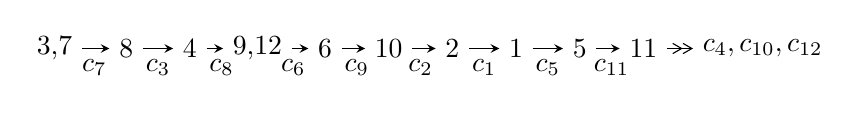
\begin{tikzpicture}[x=23pt, y=7pt]
	% node
	\node (A0) at (-1/8, 0) {3,7};
	\node (A1) at (1, 0) {8};
	\node (A2) at (2, 0) {4};
	\node (A3) at (49/16, 0) {9,12};
	\node (A4) at (33/8, 0) {6};
	\node (A5) at (41/8, 0) {10};
	\node (A6) at (49/8, 0) {2};
	\node (A7) at (57/8, 0) {1};
	\node (A8) at (65/8, 0) {5};
	\node (A9) at (73/8, 0) {11};
	\node (C1) at (1/2, -1) {$c_{7}$};
	\node (C2) at (3/2, -1) {$c_{3}$};
	\node (C3) at (5/2, -1) {$c_{8}$};
	\node (C4) at (29/8, -1) {$c_{6}$};
	\node (C5) at (37/8, -1) {$c_{9}$};
	\node (C6) at (45/8, -1) {$c_{2}$};
	\node (C7) at (53/8, -1) {$c_{1}$};
	\node (C8) at (61/8, -1) {$c_{5}$};
	\node (C9) at (69/8, -1) {$c_{11}$};
	\node (A10) at (11, 0) {$c_{4},c_{10},c_{12}$};

	% edge
	\draw[->,>=stealth]	
	(A0) edge (A1) (A1) edge (A2) (A2) edge (A3) (A3) edge (A4) (A4) edge (A5) (A5) edge (A6) (A6) edge (A7) (A7) edge (A8) (A8) edge (A9) ;
	\draw[->>,>={angle 60}]	
	(A9) edge (A10);
\end{tikzpicture} \\ 

\end{tabular} \\

\footnotetext{
The image of knot diagram is generated by the software ``\textbf{Draw programme}" developed by Andrew Bartholomew(\url{http://www.layer8.co.uk/maths/draw/index.htm\#Running-draw}), where we modified some parts for our purpose(\url{https://github.com/CATsTAILs/LinksPainter}).
}\phantom \\ \newline 
\centering \textbf{Ideals for irreducible components\footnotemark of $X_{\text{par}}$} 
 
\begin{align*}
I^u_{1}&=\langle 
261 u^{16}-101 u^{15}+\cdots+817 b+94,\;113 u^{16}+166 u^{15}+\cdots+817 a-745,\\
\phantom{I^u_{1}}&\phantom{= \langle  }u^{17}-6 u^{15}+15 u^{13}- u^{12}-15 u^{11}+5 u^{10}-5 u^9-10 u^8+24 u^7+11 u^6-18 u^5-7 u^4+4 u^3+3 u^2+u-1\rangle \\
I^u_{2}&=\langle 
-1.51873\times10^{37} u^{39}-1.89646\times10^{37} u^{38}+\cdots+1.21750\times10^{38} b-1.24577\times10^{38},\\
\phantom{I^u_{2}}&\phantom{= \langle  }2.13718\times10^{37} u^{39}+1.36142\times10^{37} u^{38}+\cdots+3.65251\times10^{38} a+1.26689\times10^{39},\;u^{40}+u^{39}+\cdots-24 u-9\rangle \\
I^u_{3}&=\langle 
- u^8+2 u^6-2 u^4- u^3+u^2+b+1,\;u^8- u^7-3 u^6+2 u^5+4 u^4-2 u^3-4 u^2+a+u+1,\\
\phantom{I^u_{3}}&\phantom{= \langle  }u^9-3 u^7+5 u^5+u^4-5 u^3- u^2+2 u+1\rangle \\
I^u_{4}&=\langle 
u^6-2 u^4- u^3+u^2+b-1,\;-2 u^9+2 u^8+5 u^7-4 u^6-8 u^5+7 u^4+8 u^3-5 u^2+a-6 u+5,\\
\phantom{I^u_{4}}&\phantom{= \langle  }u^{10}-3 u^8- u^7+4 u^6+u^5-4 u^4- u^3+3 u^2-1\rangle \\
\\
\end{align*}
\raggedright * 4 irreducible components of $\dim_{\mathbb{C}}=0$, with total 76 representations.\\
\footnotetext{All coefficients of polynomials are rational numbers. But the coefficients are sometimes approximated in decimal forms when there is not enough margin.}
\newpage
\renewcommand{\arraystretch}{1}
\centering \section*{I. $I^u_{1}= \langle 261 u^{16}-101 u^{15}+\cdots+817 b+94,\;113 u^{16}+166 u^{15}+\cdots+817 a-745,\;u^{17}-6 u^{15}+\cdots+u-1 \rangle$}
\flushleft \textbf{(i) Arc colorings}\\
\begin{tabular}{m{7pt} m{180pt} m{7pt} m{180pt} }
\flushright $a_{3}=$&$\begin{pmatrix}0\\u\end{pmatrix}$ \\
\flushright $a_{7}=$&$\begin{pmatrix}1\\0\end{pmatrix}$ \\
\flushright $a_{8}=$&$\begin{pmatrix}1\\u^2\end{pmatrix}$ \\
\flushright $a_{4}=$&$\begin{pmatrix}- u\\- u^3+u\end{pmatrix}$ \\
\flushright $a_{9}=$&$\begin{pmatrix}- u^2+1\\u^2\end{pmatrix}$ \\
\flushright $a_{12}=$&$\begin{pmatrix}-0.138311 u^{16}-0.203182 u^{15}+\cdots-0.357405 u+0.911873\\-0.319461 u^{16}+0.123623 u^{15}+\cdots+0.422277 u-0.115055\end{pmatrix}$ \\
\flushright $a_{6}=$&$\begin{pmatrix}-0.00979192 u^{16}+0.206854 u^{15}+\cdots+2.23133 u+0.728274\\-0.567931 u^{16}-0.00244798 u^{15}+\cdots-1.58262 u+0.239902\end{pmatrix}$ \\
\flushright $a_{10}=$&$\begin{pmatrix}0.297430 u^{16}+0.0917993 u^{15}+\cdots-0.151775 u+1.00367\\0.138311 u^{16}+0.203182 u^{15}+\cdots+0.357405 u+0.0881273\end{pmatrix}$ \\
\flushright $a_{2}=$&$\begin{pmatrix}-0.134639 u^{16}+0.0942472 u^{15}+\cdots+0.430845 u+0.763770\\-0.564259 u^{16}+0.294982 u^{15}+\cdots+0.205630 u+0.0917993\end{pmatrix}$ \\
\flushright $a_{1}=$&$\begin{pmatrix}-0.134639 u^{16}+0.0942472 u^{15}+\cdots+0.430845 u+0.763770\\-0.198286 u^{16}-0.0611995 u^{15}+\cdots+0.434517 u-0.00244798\end{pmatrix}$ \\
\flushright $a_{5}=$&$\begin{pmatrix}0.0917993 u^{16}+0.435741 u^{15}+\cdots+1.70624 u+0.297430\\0.203182 u^{16}+0.457772 u^{15}+\cdots-1.05018 u+0.138311\end{pmatrix}$ \\
\flushright $a_{11}=$&$\begin{pmatrix}0.297430 u^{16}+0.0917993 u^{15}+\cdots-0.151775 u+1.00367\\0.138311 u^{16}+0.203182 u^{15}+\cdots+0.357405 u+0.0881273\end{pmatrix}$\\&\end{tabular}
\flushleft \textbf{(ii) Obstruction class $= -1$}\\~\\
\flushleft \textbf{(iii) Cusp Shapes $= -\frac{33}{817} u^{16}-\frac{1856}{817} u^{15}+\cdots-\frac{7084}{817} u-\frac{8473}{817}$}\\~\\
\newpage\renewcommand{\arraystretch}{1}
\flushleft \textbf{(iv) u-Polynomials at the component}\newline \\
\begin{tabular}{m{50pt}|m{274pt}}
Crossings & \hspace{64pt}u-Polynomials at each crossing \\
\hline $$\begin{aligned}c_{1}\end{aligned}$$&$\begin{aligned}
&u^{17}+14 u^{16}+\cdots+3584 u+1024
\end{aligned}$\\
\hline $$\begin{aligned}c_{2},c_{5}\end{aligned}$$&$\begin{aligned}
&u^{17}+10 u^{16}+\cdots+160 u+32
\end{aligned}$\\
\hline $$\begin{aligned}c_{3},c_{4},c_{7}\\c_{10}\end{aligned}$$&$\begin{aligned}
&u^{17}-6 u^{15}+\cdots+u+1
\end{aligned}$\\
\hline $$\begin{aligned}c_{6}\end{aligned}$$&$\begin{aligned}
&u^{17}-6 u^{16}+\cdots-12 u+8
\end{aligned}$\\
\hline $$\begin{aligned}c_{8},c_{11}\end{aligned}$$&$\begin{aligned}
&u^{17}+12 u^{16}+\cdots+7 u+1
\end{aligned}$\\
\hline $$\begin{aligned}c_{9},c_{12}\end{aligned}$$&$\begin{aligned}
&u^{17}+2 u^{16}+\cdots+12 u+1
\end{aligned}$\\
\hline
\end{tabular}\\~\\
\newpage\renewcommand{\arraystretch}{1}
\flushleft \textbf{(v) Riley Polynomials at the component}\newline \\
\begin{tabular}{m{50pt}|m{274pt}}
Crossings & \hspace{64pt}Riley Polynomials at each crossing \\
\hline $$\begin{aligned}c_{1}\end{aligned}$$&$\begin{aligned}
&y^{17}-22 y^{16}+\cdots-4587520 y-1048576
\end{aligned}$\\
\hline $$\begin{aligned}c_{2},c_{5}\end{aligned}$$&$\begin{aligned}
&y^{17}-14 y^{16}+\cdots+3584 y-1024
\end{aligned}$\\
\hline $$\begin{aligned}c_{3},c_{4},c_{7}\\c_{10}\end{aligned}$$&$\begin{aligned}
&y^{17}-12 y^{16}+\cdots+7 y-1
\end{aligned}$\\
\hline $$\begin{aligned}c_{6}\end{aligned}$$&$\begin{aligned}
&y^{17}-6 y^{16}+\cdots+720 y-64
\end{aligned}$\\
\hline $$\begin{aligned}c_{8},c_{11}\end{aligned}$$&$\begin{aligned}
&y^{17}-12 y^{16}+\cdots+19 y-1
\end{aligned}$\\
\hline $$\begin{aligned}c_{9},c_{12}\end{aligned}$$&$\begin{aligned}
&y^{17}+24 y^{16}+\cdots+34 y-1
\end{aligned}$\\
\hline
\end{tabular}\\~\\
\newpage\flushleft \textbf{(vi) Complex Volumes and Cusp Shapes}
$$\begin{array}{c|c|c}  
\text{Solutions to }I^u_{1}& \I (\text{vol} + \sqrt{-1}CS) & \text{Cusp shape}\\
 \hline 
\begin{aligned}
u &= -0.872688 + 0.309245 I \\
a &= -1.10902 + 0.97065 I \\
b &= \phantom{-}1.22842 + 0.81409 I\end{aligned}
 & -1.17696 + 5.14107 I & -6.11359 - 6.50734 I \\ \hline\begin{aligned}
u &= -0.872688 - 0.309245 I \\
a &= -1.10902 - 0.97065 I \\
b &= \phantom{-}1.22842 - 0.81409 I\end{aligned}
 & -1.17696 - 5.14107 I & -6.11359 + 6.50734 I \\ \hline\begin{aligned}
u &= \phantom{-}0.112694 + 1.077070 I \\
a &= \phantom{-}1.37425 + 0.41818 I \\
b &= -0.905176 - 0.807152 I\end{aligned}
 & -5.24123 + 3.03176 I & -5.90001 - 2.22137 I \\ \hline\begin{aligned}
u &= \phantom{-}0.112694 - 1.077070 I \\
a &= \phantom{-}1.37425 - 0.41818 I \\
b &= -0.905176 + 0.807152 I\end{aligned}
 & -5.24123 - 3.03176 I & -5.90001 + 2.22137 I \\ \hline\begin{aligned}
u &= \phantom{-}0.770678 + 0.254682 I \\
a &= -0.350181 - 0.951046 I \\
b &= \phantom{-}1.009160 - 0.082155 I\end{aligned}
 & -0.500652 - 0.396435 I & -8.19182 + 2.68087 I \\ \hline\begin{aligned}
u &= \phantom{-}0.770678 - 0.254682 I \\
a &= -0.350181 + 0.951046 I \\
b &= \phantom{-}1.009160 + 0.082155 I\end{aligned}
 & -0.500652 + 0.396435 I & -8.19182 - 2.68087 I \\ \hline\begin{aligned}
u &= -1.220540 + 0.157617 I \\
a &= -0.501451 + 0.512731 I \\
b &= -0.500714 + 0.816049 I\end{aligned}
 & -6.48988 + 1.76820 I & -13.17903 - 1.70263 I \\ \hline\begin{aligned}
u &= -1.220540 - 0.157617 I \\
a &= -0.501451 - 0.512731 I \\
b &= -0.500714 - 0.816049 I\end{aligned}
 & -6.48988 - 1.76820 I & -13.17903 + 1.70263 I \\ \hline\begin{aligned}
u &= \phantom{-}1.251960 + 0.260556 I \\
a &= \phantom{-}0.82098 + 1.51753 I \\
b &= -1.079480 + 0.641251 I\end{aligned}
 & -4.75266 - 7.21790 I & -11.92961 + 6.92939 I \\ \hline\begin{aligned}
u &= \phantom{-}1.251960 - 0.260556 I \\
a &= \phantom{-}0.82098 - 1.51753 I \\
b &= -1.079480 - 0.641251 I\end{aligned}
 & -4.75266 + 7.21790 I & -11.92961 - 6.92939 I\\
 \hline 
 \end{array}$$\newpage$$\begin{array}{c|c|c}  
\text{Solutions to }I^u_{1}& \I (\text{vol} + \sqrt{-1}CS) & \text{Cusp shape}\\
 \hline 
\begin{aligned}
u &= \phantom{-}1.329090 + 0.472313 I \\
a &= -0.038538 + 0.181070 I \\
b &= -0.79169 - 1.20549 I\end{aligned}
 & -14.4213 - 7.4571 I & -11.51687 + 4.18112 I \\ \hline\begin{aligned}
u &= \phantom{-}1.329090 - 0.472313 I \\
a &= -0.038538 - 0.181070 I \\
b &= -0.79169 + 1.20549 I\end{aligned}
 & -14.4213 + 7.4571 I & -11.51687 - 4.18112 I \\ \hline\begin{aligned}
u &= -0.246489 + 0.489685 I \\
a &= \phantom{-}1.73580 - 0.42019 I \\
b &= -0.968967 + 0.317789 I\end{aligned}
 & \phantom{-}1.66217 - 1.14629 I & \phantom{-}1.43775 + 2.20534 I \\ \hline\begin{aligned}
u &= -0.246489 - 0.489685 I \\
a &= \phantom{-}1.73580 + 0.42019 I \\
b &= -0.968967 - 0.317789 I\end{aligned}
 & \phantom{-}1.66217 + 1.14629 I & \phantom{-}1.43775 - 2.20534 I \\ \hline\begin{aligned}
u &= -1.35873 + 0.57627 I \\
a &= \phantom{-}1.29756 - 0.84527 I \\
b &= -1.17071 - 0.90048 I\end{aligned}
 & -13.0830 + 14.9833 I & -9.98102 - 7.51290 I \\ \hline\begin{aligned}
u &= -1.35873 - 0.57627 I \\
a &= \phantom{-}1.29756 + 0.84527 I \\
b &= -1.17071 + 0.90048 I\end{aligned}
 & -13.0830 - 14.9833 I & -9.98102 + 7.51290 I \\ \hline\begin{aligned}
u &= \phantom{-}0.468027\phantom{ +0.000000I} \\
a &= \phantom{-}0.541197\phantom{ +0.000000I} \\
b &= \phantom{-}0.358302\phantom{ +0.000000I}\end{aligned}
 & -0.819496\phantom{ +0.000000I} & -12.2520\phantom{ +0.000000I}\\
 \hline 
 \end{array}$$\newpage\newpage\renewcommand{\arraystretch}{1}
\centering \section*{II. $I^u_{2}= \langle -1.52\times10^{37} u^{39}-1.90\times10^{37} u^{38}+\cdots+1.22\times10^{38} b-1.25\times10^{38},\;2.14\times10^{37} u^{39}+1.36\times10^{37} u^{38}+\cdots+3.65\times10^{38} a+1.27\times10^{39},\;u^{40}+u^{39}+\cdots-24 u-9 \rangle$}
\flushleft \textbf{(i) Arc colorings}\\
\begin{tabular}{m{7pt} m{180pt} m{7pt} m{180pt} }
\flushright $a_{3}=$&$\begin{pmatrix}0\\u\end{pmatrix}$ \\
\flushright $a_{7}=$&$\begin{pmatrix}1\\0\end{pmatrix}$ \\
\flushright $a_{8}=$&$\begin{pmatrix}1\\u^2\end{pmatrix}$ \\
\flushright $a_{4}=$&$\begin{pmatrix}- u\\- u^3+u\end{pmatrix}$ \\
\flushright $a_{9}=$&$\begin{pmatrix}- u^2+1\\u^2\end{pmatrix}$ \\
\flushright $a_{12}=$&$\begin{pmatrix}-0.0585128 u^{39}-0.0372737 u^{38}+\cdots+1.70400 u-3.46855\\0.124742 u^{39}+0.155767 u^{38}+\cdots+2.43424 u+1.02322\end{pmatrix}$ \\
\flushright $a_{6}=$&$\begin{pmatrix}-0.201855 u^{39}+0.202202 u^{38}+\cdots+6.51731 u+1.59348\\0.147685 u^{39}+0.0264282 u^{38}+\cdots+2.61080 u+0.354275\end{pmatrix}$ \\
\flushright $a_{10}=$&$\begin{pmatrix}0.0813577 u^{39}-0.202188 u^{38}+\cdots+7.28317 u+1.97309\\0.0286342 u^{39}+0.0928329 u^{38}+\cdots-3.22599 u+0.539866\end{pmatrix}$ \\
\flushright $a_{2}=$&$\begin{pmatrix}-0.200240 u^{39}-0.0544321 u^{38}+\cdots+5.36707 u-1.24072\\0.118463 u^{39}+0.127401 u^{38}+\cdots+1.05224 u+0.660498\end{pmatrix}$ \\
\flushright $a_{1}=$&$\begin{pmatrix}-0.200240 u^{39}-0.0544321 u^{38}+\cdots+5.36707 u-1.24072\\0.420625 u^{39}+0.140972 u^{38}+\cdots-0.644987 u-0.651772\end{pmatrix}$ \\
\flushright $a_{5}=$&$\begin{pmatrix}0.835765 u^{39}+0.0374218 u^{38}+\cdots-22.3043 u-11.6309\\0.114623 u^{39}+0.0818378 u^{38}+\cdots+5.71886 u-0.0603670\end{pmatrix}$ \\
\flushright $a_{11}=$&$\begin{pmatrix}0.175078 u^{39}-0.284313 u^{38}+\cdots+4.95360 u+0.359674\\-0.0140809 u^{39}+0.0620252 u^{38}+\cdots-4.27325 u+0.570666\end{pmatrix}$\\&\end{tabular}
\flushleft \textbf{(ii) Obstruction class $= -1$}\\~\\
\flushleft \textbf{(iii) Cusp Shapes $= 0.893186 u^{39}+0.382084 u^{38}+\cdots-32.1739 u-19.4647$}\\~\\
\newpage\renewcommand{\arraystretch}{1}
\flushleft \textbf{(iv) u-Polynomials at the component}\newline \\
\begin{tabular}{m{50pt}|m{274pt}}
Crossings & \hspace{64pt}u-Polynomials at each crossing \\
\hline $$\begin{aligned}c_{1}\end{aligned}$$&$\begin{aligned}
&(u^{20}+30 u^{19}+\cdots+881 u+25)^{2}
\end{aligned}$\\
\hline $$\begin{aligned}c_{2},c_{5}\end{aligned}$$&$\begin{aligned}
&(u^{20}-4 u^{19}+\cdots-9 u-5)^{2}
\end{aligned}$\\
\hline $$\begin{aligned}c_{3},c_{4},c_{7}\\c_{10}\end{aligned}$$&$\begin{aligned}
&u^{40}- u^{39}+\cdots+24 u-9
\end{aligned}$\\
\hline $$\begin{aligned}c_{6}\end{aligned}$$&$\begin{aligned}
&(u^{20}+2 u^{19}+\cdots+2 u-1)^{2}
\end{aligned}$\\
\hline $$\begin{aligned}c_{8},c_{11}\end{aligned}$$&$\begin{aligned}
&u^{40}+27 u^{39}+\cdots-702 u+81
\end{aligned}$\\
\hline $$\begin{aligned}c_{9},c_{12}\end{aligned}$$&$\begin{aligned}
&u^{40}+8 u^{39}+\cdots-241750 u-136681
\end{aligned}$\\
\hline
\end{tabular}\\~\\
\newpage\renewcommand{\arraystretch}{1}
\flushleft \textbf{(v) Riley Polynomials at the component}\newline \\
\begin{tabular}{m{50pt}|m{274pt}}
Crossings & \hspace{64pt}Riley Polynomials at each crossing \\
\hline $$\begin{aligned}c_{1}\end{aligned}$$&$\begin{aligned}
&(y^{20}-82 y^{19}+\cdots-403661 y+625)^{2}
\end{aligned}$\\
\hline $$\begin{aligned}c_{2},c_{5}\end{aligned}$$&$\begin{aligned}
&(y^{20}-30 y^{19}+\cdots-881 y+25)^{2}
\end{aligned}$\\
\hline $$\begin{aligned}c_{3},c_{4},c_{7}\\c_{10}\end{aligned}$$&$\begin{aligned}
&y^{40}-27 y^{39}+\cdots+702 y+81
\end{aligned}$\\
\hline $$\begin{aligned}c_{6}\end{aligned}$$&$\begin{aligned}
&(y^{20}-6 y^{19}+\cdots-26 y+1)^{2}
\end{aligned}$\\
\hline $$\begin{aligned}c_{8},c_{11}\end{aligned}$$&$\begin{aligned}
&y^{40}-19 y^{39}+\cdots-578178 y+6561
\end{aligned}$\\
\hline $$\begin{aligned}c_{9},c_{12}\end{aligned}$$&$\begin{aligned}
&y^{40}-2 y^{39}+\cdots+22299598078 y+18681695761
\end{aligned}$\\
\hline
\end{tabular}\\~\\
\newpage\flushleft \textbf{(vi) Complex Volumes and Cusp Shapes}
$$\begin{array}{c|c|c}  
\text{Solutions to }I^u_{2}& \I (\text{vol} + \sqrt{-1}CS) & \text{Cusp shape}\\
 \hline 
\begin{aligned}
u &= \phantom{-}0.985793 + 0.106099 I \\
a &= \phantom{-}1.47285 + 0.70515 I \\
b &= -1.313450 + 0.406280 I\end{aligned}
 & -0.81957 - 1.24696 I & -7.62468 + 0.13280 I \\ \hline\begin{aligned}
u &= \phantom{-}0.985793 - 0.106099 I \\
a &= \phantom{-}1.47285 - 0.70515 I \\
b &= -1.313450 - 0.406280 I\end{aligned}
 & -0.81957 + 1.24696 I & -7.62468 - 0.13280 I \\ \hline\begin{aligned}
u &= -0.061557 + 0.981252 I \\
a &= -1.42687 + 0.39525 I \\
b &= \phantom{-}0.740083 - 0.981052 I\end{aligned}
 & -10.10780 + 2.32175 I & -8.97701 - 0.73874 I \\ \hline\begin{aligned}
u &= -0.061557 - 0.981252 I \\
a &= -1.42687 - 0.39525 I \\
b &= \phantom{-}0.740083 + 0.981052 I\end{aligned}
 & -10.10780 - 2.32175 I & -8.97701 + 0.73874 I \\ \hline\begin{aligned}
u &= \phantom{-}0.836619 + 0.625265 I \\
a &= -1.68057 + 0.31357 I \\
b &= \phantom{-}0.745821 - 0.208249 I\end{aligned}
 & \phantom{-}1.03980 - 5.20042 I & -4.45133 + 5.57600 I \\ \hline\begin{aligned}
u &= \phantom{-}0.836619 - 0.625265 I \\
a &= -1.68057 - 0.31357 I \\
b &= \phantom{-}0.745821 + 0.208249 I\end{aligned}
 & \phantom{-}1.03980 + 5.20042 I & -4.45133 - 5.57600 I \\ \hline\begin{aligned}
u &= \phantom{-}1.092520 + 0.041392 I \\
a &= \phantom{-}0.114066 - 0.561701 I \\
b &= \phantom{-}0.687385 - 0.749134 I\end{aligned}
 & -1.84004 - 0.63402 I & -8.04331 - 0.15211 I \\ \hline\begin{aligned}
u &= \phantom{-}1.092520 - 0.041392 I \\
a &= \phantom{-}0.114066 + 0.561701 I \\
b &= \phantom{-}0.687385 + 0.749134 I\end{aligned}
 & -1.84004 + 0.63402 I & -8.04331 + 0.15211 I \\ \hline\begin{aligned}
u &= -0.671937 + 0.604612 I \\
a &= \phantom{-}0.525601 - 0.779399 I \\
b &= -1.313450 + 0.406280 I\end{aligned}
 & -0.81957 - 1.24696 I & -7.62468 + 0.13280 I \\ \hline\begin{aligned}
u &= -0.671937 - 0.604612 I \\
a &= \phantom{-}0.525601 + 0.779399 I \\
b &= -1.313450 - 0.406280 I\end{aligned}
 & -0.81957 + 1.24696 I & -7.62468 - 0.13280 I\\
 \hline 
 \end{array}$$\newpage$$\begin{array}{c|c|c}  
\text{Solutions to }I^u_{2}& \I (\text{vol} + \sqrt{-1}CS) & \text{Cusp shape}\\
 \hline 
\begin{aligned}
u &= -1.10100\phantom{ +0.000000I} \\
a &= -3.54571\phantom{ +0.000000I} \\
b &= \phantom{-}0.847094\phantom{ +0.000000I}\end{aligned}
 & -8.45151\phantom{ +0.000000I} & -8.71120\phantom{ +0.000000I} \\ \hline\begin{aligned}
u &= \phantom{-}0.850304 + 0.713148 I \\
a &= \phantom{-}1.013260 + 0.848398 I \\
b &= -0.493869\phantom{ +0.000000I}\end{aligned}
 & \phantom{-}1.03533\phantom{ +0.000000I} & -6.45138 + 0. I\phantom{ +0.000000I} \\ \hline\begin{aligned}
u &= \phantom{-}0.850304 - 0.713148 I \\
a &= \phantom{-}1.013260 - 0.848398 I \\
b &= -0.493869\phantom{ +0.000000I}\end{aligned}
 & \phantom{-}1.03533\phantom{ +0.000000I} & -6.45138 + 0. I\phantom{ +0.000000I} \\ \hline\begin{aligned}
u &= -0.562871 + 0.677759 I \\
a &= \phantom{-}1.350220 + 0.203953 I \\
b &= -0.846857\phantom{ +0.000000I}\end{aligned}
 & \phantom{-}2.60911\phantom{ +0.000000I} & \phantom{-}                -6
0.518982 + 0. 10   I\phantom{ +0.000000I} \\ \hline\begin{aligned}
u &= -0.562871 - 0.677759 I \\
a &= \phantom{-}1.350220 - 0.203953 I \\
b &= -0.846857\phantom{ +0.000000I}\end{aligned}
 & \phantom{-}2.60911\phantom{ +0.000000I} & \phantom{-}                -6
0.518982 + 0. 10   I\phantom{ +0.000000I} \\ \hline\begin{aligned}
u &= -0.069227 + 1.125560 I \\
a &= -1.36033 + 0.39893 I \\
b &= \phantom{-}1.077500 - 0.827760 I\end{aligned}
 & -9.04644 - 8.94980 I & -7.77982 + 5.10458 I \\ \hline\begin{aligned}
u &= -0.069227 - 1.125560 I \\
a &= -1.36033 - 0.39893 I \\
b &= \phantom{-}1.077500 + 0.827760 I\end{aligned}
 & -9.04644 + 8.94980 I & -7.77982 - 5.10458 I \\ \hline\begin{aligned}
u &= -1.093460 + 0.370616 I \\
a &= -0.98200 + 1.09858 I \\
b &= \phantom{-}1.011700 + 0.632363 I\end{aligned}
 & -0.78834 + 4.67433 I & -5.30649 - 6.82521 I \\ \hline\begin{aligned}
u &= -1.093460 - 0.370616 I \\
a &= -0.98200 - 1.09858 I \\
b &= \phantom{-}1.011700 - 0.632363 I\end{aligned}
 & -0.78834 - 4.67433 I & -5.30649 + 6.82521 I \\ \hline\begin{aligned}
u &= -1.157600 + 0.120447 I \\
a &= -0.042441 - 0.362661 I \\
b &= -0.656124 - 1.053570 I\end{aligned}
 & -3.80624 + 5.08920 I & -12.34652 - 4.90346 I\\
 \hline 
 \end{array}$$\newpage$$\begin{array}{c|c|c}  
\text{Solutions to }I^u_{2}& \I (\text{vol} + \sqrt{-1}CS) & \text{Cusp shape}\\
 \hline 
\begin{aligned}
u &= -1.157600 - 0.120447 I \\
a &= -0.042441 + 0.362661 I \\
b &= -0.656124 + 1.053570 I\end{aligned}
 & -3.80624 - 5.08920 I & -12.34652 + 4.90346 I \\ \hline\begin{aligned}
u &= \phantom{-}1.043330 + 0.515865 I \\
a &= \phantom{-}0.976781 + 0.822046 I \\
b &= -0.656124 + 1.053570 I\end{aligned}
 & -3.80624 - 5.08920 I & -12.34652 + 4.90346 I \\ \hline\begin{aligned}
u &= \phantom{-}1.043330 - 0.515865 I \\
a &= \phantom{-}0.976781 - 0.822046 I \\
b &= -0.656124 - 1.053570 I\end{aligned}
 & -3.80624 + 5.08920 I & -12.34652 - 4.90346 I \\ \hline\begin{aligned}
u &= -0.746386\phantom{ +0.000000I} \\
a &= -4.63725\phantom{ +0.000000I} \\
b &= -0.254182\phantom{ +0.000000I}\end{aligned}
 & -7.16640\phantom{ +0.000000I} & -21.4380\phantom{ +0.000000I} \\ \hline\begin{aligned}
u &= -1.096590 + 0.652317 I \\
a &= -0.831505 + 0.847751 I \\
b &= \phantom{-}0.745821 + 0.208249 I\end{aligned}
 & \phantom{-}1.03980 + 5.20042 I & -4.45133 - 5.57600 I \\ \hline\begin{aligned}
u &= -1.096590 - 0.652317 I \\
a &= -0.831505 - 0.847751 I \\
b &= \phantom{-}0.745821 - 0.208249 I\end{aligned}
 & \phantom{-}1.03980 - 5.20042 I & -4.45133 + 5.57600 I \\ \hline\begin{aligned}
u &= \phantom{-}0.331219 + 0.637366 I \\
a &= -0.382754 - 0.453408 I \\
b &= \phantom{-}0.687385 + 0.749134 I\end{aligned}
 & -1.84004 + 0.63402 I & -8.04331 + 0.15211 I \\ \hline\begin{aligned}
u &= \phantom{-}0.331219 - 0.637366 I \\
a &= -0.382754 + 0.453408 I \\
b &= \phantom{-}0.687385 - 0.749134 I\end{aligned}
 & -1.84004 - 0.63402 I & -8.04331 - 0.15211 I \\ \hline\begin{aligned}
u &= -1.300800 + 0.543331 I \\
a &= \phantom{-}1.58939 - 0.86240 I \\
b &= -0.919010 - 0.840072 I\end{aligned}
 & -13.8803 + 3.1384 I & -10.93015 + 0. I\phantom{ +0.000000I} \\ \hline\begin{aligned}
u &= -1.300800 - 0.543331 I \\
a &= \phantom{-}1.58939 + 0.86240 I \\
b &= -0.919010 + 0.840072 I\end{aligned}
 & -13.8803 - 3.1384 I & -10.93015 + 0. I\phantom{ +0.000000I}\\
 \hline 
 \end{array}$$\newpage$$\begin{array}{c|c|c}  
\text{Solutions to }I^u_{2}& \I (\text{vol} + \sqrt{-1}CS) & \text{Cusp shape}\\
 \hline 
\begin{aligned}
u &= \phantom{-}1.33349 + 0.57768 I \\
a &= -1.40702 - 0.79123 I \\
b &= \phantom{-}1.077500 - 0.827760 I\end{aligned}
 & -9.04644 - 8.94980 I & \phantom{-0.000000 } 0 \\ \hline\begin{aligned}
u &= \phantom{-}1.33349 - 0.57768 I \\
a &= -1.40702 + 0.79123 I \\
b &= \phantom{-}1.077500 + 0.827760 I\end{aligned}
 & -9.04644 + 8.94980 I & \phantom{-0.000000 } 0 \\ \hline\begin{aligned}
u &= -1.39353 + 0.44049 I \\
a &= -0.061607 + 0.191617 I \\
b &= \phantom{-}0.740083 - 0.981052 I\end{aligned}
 & -10.10780 + 2.32175 I & \phantom{-0.000000 } 0 \\ \hline\begin{aligned}
u &= -1.39353 - 0.44049 I \\
a &= -0.061607 - 0.191617 I \\
b &= \phantom{-}0.740083 + 0.981052 I\end{aligned}
 & -10.10780 - 2.32175 I & \phantom{-0.000000 } 0 \\ \hline\begin{aligned}
u &= -1.47294\phantom{ +0.000000I} \\
a &= -0.409227\phantom{ +0.000000I} \\
b &= -0.254182\phantom{ +0.000000I}\end{aligned}
 & -7.16640\phantom{ +0.000000I} & -21.4380\phantom{ +0.000000I} \\ \hline\begin{aligned}
u &= \phantom{-}1.47987\phantom{ +0.000000I} \\
a &= \phantom{-}0.579170\phantom{ +0.000000I} \\
b &= \phantom{-}0.847094\phantom{ +0.000000I}\end{aligned}
 & -8.45151\phantom{ +0.000000I} & -8.71120\phantom{ +0.000000I} \\ \hline\begin{aligned}
u &= \phantom{-}1.44287 + 0.49042 I \\
a &= \phantom{-}0.097964 + 0.290556 I \\
b &= -0.919010 - 0.840072 I\end{aligned}
 & -13.8803 + 3.1384 I & \phantom{-0.000000 } 0 \\ \hline\begin{aligned}
u &= \phantom{-}1.44287 - 0.49042 I \\
a &= \phantom{-}0.097964 - 0.290556 I \\
b &= -0.919010 + 0.840072 I\end{aligned}
 & -13.8803 - 3.1384 I & \phantom{-0.000000 } 0 \\ \hline\begin{aligned}
u &= -0.088339 + 0.296040 I \\
a &= -3.29187 + 1.03172 I \\
b &= \phantom{-}1.011700 + 0.632363 I\end{aligned}
 & -0.78834 + 4.67433 I & -5.30649 - 6.82521 I \\ \hline\begin{aligned}
u &= -0.088339 - 0.296040 I \\
a &= -3.29187 - 1.03172 I \\
b &= \phantom{-}1.011700 - 0.632363 I\end{aligned}
 & -0.78834 - 4.67433 I & -5.30649 + 6.82521 I\\
 \hline 
 \end{array}$$\newpage\newpage\renewcommand{\arraystretch}{1}
\centering \section*{III. $I^u_{3}= \langle - u^8+2 u^6-2 u^4- u^3+u^2+b+1,\;u^8- u^7+\cdots+a+1,\;u^9-3 u^7+5 u^5+u^4-5 u^3- u^2+2 u+1 \rangle$}
\flushleft \textbf{(i) Arc colorings}\\
\begin{tabular}{m{7pt} m{180pt} m{7pt} m{180pt} }
\flushright $a_{3}=$&$\begin{pmatrix}0\\u\end{pmatrix}$ \\
\flushright $a_{7}=$&$\begin{pmatrix}1\\0\end{pmatrix}$ \\
\flushright $a_{8}=$&$\begin{pmatrix}1\\u^2\end{pmatrix}$ \\
\flushright $a_{4}=$&$\begin{pmatrix}- u\\- u^3+u\end{pmatrix}$ \\
\flushright $a_{9}=$&$\begin{pmatrix}- u^2+1\\u^2\end{pmatrix}$ \\
\flushright $a_{12}=$&$\begin{pmatrix}- u^8+u^7+3 u^6-2 u^5-4 u^4+2 u^3+4 u^2- u-1\\u^8-2 u^6+2 u^4+u^3- u^2-1\end{pmatrix}$ \\
\flushright $a_{6}=$&$\begin{pmatrix}u^8-3 u^6+5 u^4-5 u^2+2\\- u^8+2 u^6- u^5-3 u^4+u^3+2 u^2-2 u\end{pmatrix}$ \\
\flushright $a_{10}=$&$\begin{pmatrix}u^6- u^5-2 u^4+u^3+2 u^2- u-1\\u^8- u^7-3 u^6+2 u^5+4 u^4-2 u^3-3 u^2+u\end{pmatrix}$ \\
\flushright $a_{2}=$&$\begin{pmatrix}- u^8+u^7+3 u^6-2 u^5-5 u^4+2 u^3+5 u^2- u-2\\u^8-2 u^6+2 u^4+u^3- u^2+u-1\end{pmatrix}$ \\
\flushright $a_{1}=$&$\begin{pmatrix}- u^8+u^7+3 u^6-2 u^5-5 u^4+2 u^3+5 u^2- u-2\\u^8- u^7-2 u^6+2 u^5+3 u^4-2 u^3-2 u^2+2 u\end{pmatrix}$ \\
\flushright $a_{5}=$&$\begin{pmatrix}u^7- u^6-2 u^5+u^4+3 u^3- u^2-2 u\\- u^8+2 u^6-3 u^4+2 u^2- u-1\end{pmatrix}$ \\
\flushright $a_{11}=$&$\begin{pmatrix}u^6- u^5-2 u^4+u^3+3 u^2- u-1\\u^8- u^7-3 u^6+2 u^5+5 u^4-2 u^3-4 u^2+u\end{pmatrix}$\\&\end{tabular}
\flushleft \textbf{(ii) Obstruction class $= 1$}\\~\\
\flushleft \textbf{(iii) Cusp Shapes $= u^8+6 u^7-3 u^6-10 u^5+4 u^4+15 u^3+3 u^2-11 u-7$}\\~\\
\newpage\renewcommand{\arraystretch}{1}
\flushleft \textbf{(iv) u-Polynomials at the component}\newline \\
\begin{tabular}{m{50pt}|m{274pt}}
Crossings & \hspace{64pt}u-Polynomials at each crossing \\
\hline $$\begin{aligned}c_{1}\end{aligned}$$&$\begin{aligned}
&u^9-9 u^8+28 u^7-51 u^6+59 u^5-48 u^4+29 u^3-14 u^2+5 u-1
\end{aligned}$\\
\hline $$\begin{aligned}c_{2}\end{aligned}$$&$\begin{aligned}
&u^9- u^8-4 u^7+u^6+5 u^5-2 u^4-3 u^3+2 u^2+u-1
\end{aligned}$\\
\hline $$\begin{aligned}c_{3},c_{10}\end{aligned}$$&$\begin{aligned}
&u^9-3 u^7+5 u^5- u^4-5 u^3+u^2+2 u-1
\end{aligned}$\\
\hline $$\begin{aligned}c_{4},c_{7}\end{aligned}$$&$\begin{aligned}
&u^9-3 u^7+5 u^5+u^4-5 u^3- u^2+2 u+1
\end{aligned}$\\
\hline $$\begin{aligned}c_{5}\end{aligned}$$&$\begin{aligned}
&u^9+u^8-4 u^7- u^6+5 u^5+2 u^4-3 u^3-2 u^2+u+1
\end{aligned}$\\
\hline $$\begin{aligned}c_{6}\end{aligned}$$&$\begin{aligned}
&u^9+u^8-2 u^7-3 u^6+2 u^5+5 u^4- u^3-4 u^2+u+1
\end{aligned}$\\
\hline $$\begin{aligned}c_{8},c_{11}\end{aligned}$$&$\begin{aligned}
&u^9+6 u^8+19 u^7+40 u^6+59 u^5+63 u^4+47 u^3+23 u^2+6 u+1
\end{aligned}$\\
\hline $$\begin{aligned}c_{9},c_{12}\end{aligned}$$&$\begin{aligned}
&u^9+4 u^8+3 u^7- u^6-6 u^5-3 u^4- u^3+2 u^2+u+1
\end{aligned}$\\
\hline
\end{tabular}\\~\\
\newpage\renewcommand{\arraystretch}{1}
\flushleft \textbf{(v) Riley Polynomials at the component}\newline \\
\begin{tabular}{m{50pt}|m{274pt}}
Crossings & \hspace{64pt}Riley Polynomials at each crossing \\
\hline $$\begin{aligned}c_{1}\end{aligned}$$&$\begin{aligned}
&y^9-25 y^8-16 y^7-103 y^6-33 y^5-48 y^4-15 y^3-2 y^2-3 y-1
\end{aligned}$\\
\hline $$\begin{aligned}c_{2},c_{5}\end{aligned}$$&$\begin{aligned}
&y^9-9 y^8+28 y^7-51 y^6+59 y^5-48 y^4+29 y^3-14 y^2+5 y-1
\end{aligned}$\\
\hline $$\begin{aligned}c_{3},c_{4},c_{7}\\c_{10}\end{aligned}$$&$\begin{aligned}
&y^9-6 y^8+19 y^7-40 y^6+59 y^5-63 y^4+47 y^3-23 y^2+6 y-1
\end{aligned}$\\
\hline $$\begin{aligned}c_{6}\end{aligned}$$&$\begin{aligned}
&y^9-5 y^8+14 y^7-29 y^6+48 y^5-59 y^4+51 y^3-28 y^2+9 y-1
\end{aligned}$\\
\hline $$\begin{aligned}c_{8},c_{11}\end{aligned}$$&$\begin{aligned}
&y^9+2 y^8- y^7-20 y^6-37 y^5-47 y^4-61 y^3-91 y^2-10 y-1
\end{aligned}$\\
\hline $$\begin{aligned}c_{9},c_{12}\end{aligned}$$&$\begin{aligned}
&y^9-10 y^8+5 y^7-15 y^6+10 y^5+5 y^4+3 y^3-3 y-1
\end{aligned}$\\
\hline
\end{tabular}\\~\\
\newpage\flushleft \textbf{(vi) Complex Volumes and Cusp Shapes}
$$\begin{array}{c|c|c}  
\text{Solutions to }I^u_{3}& \I (\text{vol} + \sqrt{-1}CS) & \text{Cusp shape}\\
 \hline 
\begin{aligned}
u &= \phantom{-}1.022180 + 0.325067 I \\
a &= \phantom{-}0.587091 + 1.128900 I \\
b &= -0.846738 + 0.986047 I\end{aligned}
 & -2.29340 - 6.07855 I & -8.47383 + 8.86704 I \\ \hline\begin{aligned}
u &= \phantom{-}1.022180 - 0.325067 I \\
a &= \phantom{-}0.587091 - 1.128900 I \\
b &= -0.846738 - 0.986047 I\end{aligned}
 & -2.29340 + 6.07855 I & -8.47383 - 8.86704 I \\ \hline\begin{aligned}
u &= -0.915990 + 0.694675 I \\
a &= -1.58210 + 0.48658 I \\
b &= \phantom{-}0.993839 + 0.427672 I\end{aligned}
 & \phantom{-}1.17777 + 6.95533 I & -4.27023 - 9.54243 I \\ \hline\begin{aligned}
u &= -0.915990 - 0.694675 I \\
a &= -1.58210 - 0.48658 I \\
b &= \phantom{-}0.993839 - 0.427672 I\end{aligned}
 & \phantom{-}1.17777 - 6.95533 I & -4.27023 + 9.54243 I \\ \hline\begin{aligned}
u &= \phantom{-}1.047510 + 0.647735 I \\
a &= -0.881374 - 0.604152 I \\
b &= \phantom{-}0.781614 + 0.355685 I\end{aligned}
 & \phantom{-}0.33154 - 3.66672 I & -8.46619 + 1.40357 I \\ \hline\begin{aligned}
u &= \phantom{-}1.047510 - 0.647735 I \\
a &= -0.881374 + 0.604152 I \\
b &= \phantom{-}0.781614 - 0.355685 I\end{aligned}
 & \phantom{-}0.33154 + 3.66672 I & -8.46619 - 1.40357 I \\ \hline\begin{aligned}
u &= -1.31380\phantom{ +0.000000I} \\
a &= -1.61123\phantom{ +0.000000I} \\
b &= -0.443802\phantom{ +0.000000I}\end{aligned}
 & -9.54268\phantom{ +0.000000I} & -17.4150\phantom{ +0.000000I} \\ \hline\begin{aligned}
u &= -0.496798 + 0.288456 I \\
a &= \phantom{-}0.182003 - 0.761275 I \\
b &= -1.206810 + 0.297957 I\end{aligned}
 & \phantom{-}0.620620 - 0.259550 I & -1.58232 - 1.92541 I \\ \hline\begin{aligned}
u &= -0.496798 - 0.288456 I \\
a &= \phantom{-}0.182003 + 0.761275 I \\
b &= -1.206810 - 0.297957 I\end{aligned}
 & \phantom{-}0.620620 + 0.259550 I & -1.58232 + 1.92541 I\\
 \hline 
 \end{array}$$\newpage\newpage\renewcommand{\arraystretch}{1}
\centering \section*{IV. $I^u_{4}= \langle u^6-2 u^4- u^3+u^2+b-1,\;-2 u^9+2 u^8+\cdots+a+5,\;u^{10}-3 u^8- u^7+4 u^6+u^5-4 u^4- u^3+3 u^2-1 \rangle$}
\flushleft \textbf{(i) Arc colorings}\\
\begin{tabular}{m{7pt} m{180pt} m{7pt} m{180pt} }
\flushright $a_{3}=$&$\begin{pmatrix}0\\u\end{pmatrix}$ \\
\flushright $a_{7}=$&$\begin{pmatrix}1\\0\end{pmatrix}$ \\
\flushright $a_{8}=$&$\begin{pmatrix}1\\u^2\end{pmatrix}$ \\
\flushright $a_{4}=$&$\begin{pmatrix}- u\\- u^3+u\end{pmatrix}$ \\
\flushright $a_{9}=$&$\begin{pmatrix}- u^2+1\\u^2\end{pmatrix}$ \\
\flushright $a_{12}=$&$\begin{pmatrix}2 u^9-2 u^8-5 u^7+4 u^6+8 u^5-7 u^4-8 u^3+5 u^2+6 u-5\\- u^6+2 u^4+u^3- u^2+1\end{pmatrix}$ \\
\flushright $a_{6}=$&$\begin{pmatrix}2 u^9-5 u^7-2 u^6+5 u^5+u^4-4 u^3- u^2+3 u-1\\- u^9- u^8+2 u^7+3 u^6-2 u^4+u^3+2 u^2\end{pmatrix}$ \\
\flushright $a_{10}=$&$\begin{pmatrix}-2 u^9+u^8+5 u^7-6 u^5+u^4+5 u^3-2 u^2-4 u+3\\u^9+u^8-2 u^7-4 u^6+u^5+3 u^4- u^3-2 u^2+u+1\end{pmatrix}$ \\
\flushright $a_{2}=$&$\begin{pmatrix}2 u^9- u^8-5 u^7+u^6+7 u^5-3 u^4-7 u^3+2 u^2+5 u-3\\- u^6+2 u^4+u^3- u^2+u+1\end{pmatrix}$ \\
\flushright $a_{1}=$&$\begin{pmatrix}2 u^9- u^8-5 u^7+u^6+7 u^5-3 u^4-7 u^3+2 u^2+5 u-3\\- u^9+2 u^7-2 u^5+2 u^4+3 u^3- u^2- u+2\end{pmatrix}$ \\
\flushright $a_{5}=$&$\begin{pmatrix}-2 u^9+2 u^8+5 u^7-3 u^6-8 u^5+4 u^4+7 u^3-3 u^2-5 u+4\\-2 u^9- u^8+5 u^7+4 u^6-4 u^5-3 u^4+4 u^3+3 u^2-2 u-1\end{pmatrix}$ \\
\flushright $a_{11}=$&$\begin{pmatrix}-2 u^9+u^8+5 u^7-6 u^5+u^4+5 u^3-2 u^2-4 u+2\\u^9+u^8-2 u^7-4 u^6+u^5+3 u^4- u^3-3 u^2+u+2\end{pmatrix}$\\&\end{tabular}
\flushleft \textbf{(ii) Obstruction class $= 1$}\\~\\
\flushleft \textbf{(iii) Cusp Shapes $= -5 u^9+4 u^8+15 u^7-2 u^6-24 u^5+u^4+19 u^3-2 u^2-14 u-1$}\\~\\
\newpage\renewcommand{\arraystretch}{1}
\flushleft \textbf{(iv) u-Polynomials at the component}\newline \\
\begin{tabular}{m{50pt}|m{274pt}}
Crossings & \hspace{64pt}u-Polynomials at each crossing \\
\hline $$\begin{aligned}c_{1}\end{aligned}$$&$\begin{aligned}
&(u^5-5 u^4+8 u^3-7 u^2+3 u-1)^2
\end{aligned}$\\
\hline $$\begin{aligned}c_{2}\end{aligned}$$&$\begin{aligned}
&(u^5+u^4-2 u^3- u^2+u+1)^2
\end{aligned}$\\
\hline $$\begin{aligned}c_{3},c_{10}\end{aligned}$$&$\begin{aligned}
&u^{10}-3 u^8+u^7+4 u^6- u^5-4 u^4+u^3+3 u^2-1
\end{aligned}$\\
\hline $$\begin{aligned}c_{4},c_{7}\end{aligned}$$&$\begin{aligned}
&u^{10}-3 u^8- u^7+4 u^6+u^5-4 u^4- u^3+3 u^2-1
\end{aligned}$\\
\hline $$\begin{aligned}c_{5}\end{aligned}$$&$\begin{aligned}
&(u^5- u^4-2 u^3+u^2+u-1)^2
\end{aligned}$\\
\hline $$\begin{aligned}c_{6}\end{aligned}$$&$\begin{aligned}
&(u^5- u^4- u^3+2 u^2+u-1)^2
\end{aligned}$\\
\hline $$\begin{aligned}c_{8},c_{11}\end{aligned}$$&$\begin{aligned}
&u^{10}+6 u^9+\cdots+6 u+1
\end{aligned}$\\
\hline $$\begin{aligned}c_{9},c_{12}\end{aligned}$$&$\begin{aligned}
&u^{10}+u^9-6 u^8+4 u^7+5 u^6-11 u^5+5 u^4+4 u^3-7 u^2+4 u-1
\end{aligned}$\\
\hline
\end{tabular}\\~\\
\newpage\renewcommand{\arraystretch}{1}
\flushleft \textbf{(v) Riley Polynomials at the component}\newline \\
\begin{tabular}{m{50pt}|m{274pt}}
Crossings & \hspace{64pt}Riley Polynomials at each crossing \\
\hline $$\begin{aligned}c_{1}\end{aligned}$$&$\begin{aligned}
&(y^5-9 y^4-11 y^2-5 y-1)^2
\end{aligned}$\\
\hline $$\begin{aligned}c_{2},c_{5}\end{aligned}$$&$\begin{aligned}
&(y^5-5 y^4+8 y^3-7 y^2+3 y-1)^2
\end{aligned}$\\
\hline $$\begin{aligned}c_{3},c_{4},c_{7}\\c_{10}\end{aligned}$$&$\begin{aligned}
&y^{10}-6 y^9+\cdots-6 y+1
\end{aligned}$\\
\hline $$\begin{aligned}c_{6}\end{aligned}$$&$\begin{aligned}
&(y^5-3 y^4+7 y^3-8 y^2+5 y-1)^2
\end{aligned}$\\
\hline $$\begin{aligned}c_{8},c_{11}\end{aligned}$$&$\begin{aligned}
&y^{10}-2 y^9+\cdots-2 y+1
\end{aligned}$\\
\hline $$\begin{aligned}c_{9},c_{12}\end{aligned}$$&$\begin{aligned}
&y^{10}-13 y^9+38 y^8-44 y^7+31 y^6-29 y^5+23 y^4-8 y^3+7 y^2-2 y+1
\end{aligned}$\\
\hline
\end{tabular}\\~\\
\newpage\flushleft \textbf{(vi) Complex Volumes and Cusp Shapes}
$$\begin{array}{c|c|c}  
\text{Solutions to }I^u_{4}& \I (\text{vol} + \sqrt{-1}CS) & \text{Cusp shape}\\
 \hline 
\begin{aligned}
u &= \phantom{-}0.650832 + 0.640961 I \\
a &= \phantom{-}2.13970 + 0.29477 I \\
b &= -0.904429 + 0.339760 I\end{aligned}
 & \phantom{-}1.57933 - 1.42206 I & -3.99937 + 3.89082 I \\ \hline\begin{aligned}
u &= \phantom{-}0.650832 - 0.640961 I \\
a &= \phantom{-}2.13970 - 0.29477 I \\
b &= -0.904429 - 0.339760 I\end{aligned}
 & \phantom{-}1.57933 + 1.42206 I & -3.99937 - 3.89082 I \\ \hline\begin{aligned}
u &= -0.779988 + 0.768157 I \\
a &= \phantom{-}0.896252 - 0.611916 I \\
b &= -0.904429 + 0.339760 I\end{aligned}
 & \phantom{-}1.57933 - 1.42206 I & -3.99937 + 3.89082 I \\ \hline\begin{aligned}
u &= -0.779988 - 0.768157 I \\
a &= \phantom{-}0.896252 + 0.611916 I \\
b &= -0.904429 - 0.339760 I\end{aligned}
 & \phantom{-}1.57933 + 1.42206 I & -3.99937 - 3.89082 I \\ \hline\begin{aligned}
u &= \phantom{-}0.799959 + 0.294870 I \\
a &= -0.603978 - 0.208555 I \\
b &= \phantom{-}1.116850 + 0.784420 I\end{aligned}
 & -1.44657 + 3.45949 I & -8.68875 - 2.10393 I \\ \hline\begin{aligned}
u &= \phantom{-}0.799959 - 0.294870 I \\
a &= -0.603978 + 0.208555 I \\
b &= \phantom{-}1.116850 - 0.784420 I\end{aligned}
 & -1.44657 - 3.45949 I & -8.68875 + 2.10393 I \\ \hline\begin{aligned}
u &= -1.100530 + 0.405664 I \\
a &= -0.894237 + 0.771397 I \\
b &= \phantom{-}1.116850 + 0.784420 I\end{aligned}
 & -1.44657 + 3.45949 I & -8.68875 - 2.10393 I \\ \hline\begin{aligned}
u &= -1.100530 - 0.405664 I \\
a &= -0.894237 - 0.771397 I \\
b &= \phantom{-}1.116850 - 0.784420 I\end{aligned}
 & -1.44657 - 3.45949 I & -8.68875 + 2.10393 I \\ \hline\begin{aligned}
u &= -0.658694\phantom{ +0.000000I} \\
a &= -6.32803\phantom{ +0.000000I} \\
b &= \phantom{-}0.575152\phantom{ +0.000000I}\end{aligned}
 & -6.84525\phantom{ +0.000000I} & \phantom{-}4.37620\phantom{ +0.000000I} \\ \hline\begin{aligned}
u &= \phantom{-}1.51815\phantom{ +0.000000I} \\
a &= \phantom{-}0.252548\phantom{ +0.000000I} \\
b &= \phantom{-}0.575152\phantom{ +0.000000I}\end{aligned}
 & -6.84525\phantom{ +0.000000I} & \phantom{-}4.37620\phantom{ +0.000000I}\\
 \hline 
 \end{array}$$\newpage
\newpage\renewcommand{\arraystretch}{1}
\centering \section*{ V. u-Polynomials}
\begin{tabular}{m{50pt}|m{274pt}}
Crossings & \hspace{64pt}u-Polynomials at each crossing \\
\hline $$\begin{aligned}c_{1}\end{aligned}$$&$\begin{aligned}
&(u^5-5 u^4+8 u^3-7 u^2+3 u-1)^2\\
&\cdot(u^9-9 u^8+28 u^7-51 u^6+59 u^5-48 u^4+29 u^3-14 u^2+5 u-1)\\
&\cdot(u^{17}+14 u^{16}+\cdots+3584 u+1024)(u^{20}+30 u^{19}+\cdots+881 u+25)^{2}
\end{aligned}$\\
\hline $$\begin{aligned}c_{2}\end{aligned}$$&$\begin{aligned}
&(u^5+u^4-2 u^3- u^2+u+1)^2\\
&\cdot(u^9- u^8-4 u^7+u^6+5 u^5-2 u^4-3 u^3+2 u^2+u-1)\\
&\cdot(u^{17}+10 u^{16}+\cdots+160 u+32)(u^{20}-4 u^{19}+\cdots-9 u-5)^{2}
\end{aligned}$\\
\hline $$\begin{aligned}c_{3},c_{10}\end{aligned}$$&$\begin{aligned}
&(u^9-3 u^7+5 u^5- u^4-5 u^3+u^2+2 u-1)\\
&\cdot(u^{10}-3 u^8+\cdots+3 u^2-1)(u^{17}-6 u^{15}+\cdots+u+1)\\
&\cdot(u^{40}- u^{39}+\cdots+24 u-9)
\end{aligned}$\\
\hline $$\begin{aligned}c_{4},c_{7}\end{aligned}$$&$\begin{aligned}
&(u^9-3 u^7+5 u^5+u^4-5 u^3- u^2+2 u+1)\\
&\cdot(u^{10}-3 u^8+\cdots+3 u^2-1)(u^{17}-6 u^{15}+\cdots+u+1)\\
&\cdot(u^{40}- u^{39}+\cdots+24 u-9)
\end{aligned}$\\
\hline $$\begin{aligned}c_{5}\end{aligned}$$&$\begin{aligned}
&(u^5- u^4-2 u^3+u^2+u-1)^2\\
&\cdot(u^9+u^8-4 u^7- u^6+5 u^5+2 u^4-3 u^3-2 u^2+u+1)\\
&\cdot(u^{17}+10 u^{16}+\cdots+160 u+32)(u^{20}-4 u^{19}+\cdots-9 u-5)^{2}
\end{aligned}$\\
\hline $$\begin{aligned}c_{6}\end{aligned}$$&$\begin{aligned}
&(u^5- u^4- u^3+2 u^2+u-1)^2\\
&\cdot(u^9+u^8-2 u^7-3 u^6+2 u^5+5 u^4- u^3-4 u^2+u+1)\\
&\cdot(u^{17}-6 u^{16}+\cdots-12 u+8)(u^{20}+2 u^{19}+\cdots+2 u-1)^{2}
\end{aligned}$\\
\hline $$\begin{aligned}c_{8},c_{11}\end{aligned}$$&$\begin{aligned}
&(u^9+6 u^8+19 u^7+40 u^6+59 u^5+63 u^4+47 u^3+23 u^2+6 u+1)\\
&\cdot(u^{10}+6 u^9+\cdots+6 u+1)(u^{17}+12 u^{16}+\cdots+7 u+1)\\
&\cdot(u^{40}+27 u^{39}+\cdots-702 u+81)
\end{aligned}$\\
\hline $$\begin{aligned}c_{9},c_{12}\end{aligned}$$&$\begin{aligned}
&(u^9+4 u^8+3 u^7- u^6-6 u^5-3 u^4- u^3+2 u^2+u+1)\\
&\cdot(u^{10}+u^9-6 u^8+4 u^7+5 u^6-11 u^5+5 u^4+4 u^3-7 u^2+4 u-1)\\
&\cdot(u^{17}+2 u^{16}+\cdots+12 u+1)(u^{40}+8 u^{39}+\cdots-241750 u-136681)
\end{aligned}$\\
\hline
\end{tabular}\newpage\renewcommand{\arraystretch}{1}
\centering \section*{ VI. Riley Polynomials}
\begin{tabular}{m{50pt}|m{274pt}}
Crossings & \hspace{64pt}Riley Polynomials at each crossing \\
\hline $$\begin{aligned}c_{1}\end{aligned}$$&$\begin{aligned}
&(y^5-9 y^4-11 y^2-5 y-1)^2\\
&\cdot(y^9-25 y^8-16 y^7-103 y^6-33 y^5-48 y^4-15 y^3-2 y^2-3 y-1)\\
&\cdot(y^{17}-22 y^{16}+\cdots-4587520 y-1048576)\\
&\cdot(y^{20}-82 y^{19}+\cdots-403661 y+625)^{2}
\end{aligned}$\\
\hline $$\begin{aligned}c_{2},c_{5}\end{aligned}$$&$\begin{aligned}
&(y^5-5 y^4+8 y^3-7 y^2+3 y-1)^2\\
&\cdot(y^9-9 y^8+28 y^7-51 y^6+59 y^5-48 y^4+29 y^3-14 y^2+5 y-1)\\
&\cdot(y^{17}-14 y^{16}+\cdots+3584 y-1024)(y^{20}-30 y^{19}+\cdots-881 y+25)^{2}
\end{aligned}$\\
\hline $$\begin{aligned}c_{3},c_{4},c_{7}\\c_{10}\end{aligned}$$&$\begin{aligned}
&(y^9-6 y^8+19 y^7-40 y^6+59 y^5-63 y^4+47 y^3-23 y^2+6 y-1)\\
&\cdot(y^{10}-6 y^9+\cdots-6 y+1)(y^{17}-12 y^{16}+\cdots+7 y-1)\\
&\cdot(y^{40}-27 y^{39}+\cdots+702 y+81)
\end{aligned}$\\
\hline $$\begin{aligned}c_{6}\end{aligned}$$&$\begin{aligned}
&(y^5-3 y^4+7 y^3-8 y^2+5 y-1)^2\\
&\cdot(y^9-5 y^8+14 y^7-29 y^6+48 y^5-59 y^4+51 y^3-28 y^2+9 y-1)\\
&\cdot(y^{17}-6 y^{16}+\cdots+720 y-64)(y^{20}-6 y^{19}+\cdots-26 y+1)^{2}
\end{aligned}$\\
\hline $$\begin{aligned}c_{8},c_{11}\end{aligned}$$&$\begin{aligned}
&(y^9+2 y^8- y^7-20 y^6-37 y^5-47 y^4-61 y^3-91 y^2-10 y-1)\\
&\cdot(y^{10}-2 y^9+\cdots-2 y+1)(y^{17}-12 y^{16}+\cdots+19 y-1)\\
&\cdot(y^{40}-19 y^{39}+\cdots-578178 y+6561)
\end{aligned}$\\
\hline $$\begin{aligned}c_{9},c_{12}\end{aligned}$$&$\begin{aligned}
&(y^9-10 y^8+5 y^7-15 y^6+10 y^5+5 y^4+3 y^3-3 y-1)\\
&\cdot(y^{10}-13 y^9+38 y^8-44 y^7+31 y^6-29 y^5+23 y^4-8 y^3+7 y^2-2 y+1)\\
&\cdot(y^{17}+24 y^{16}+\cdots+34 y-1)\\
&\cdot(y^{40}-2 y^{39}+\cdots+22299598078 y+18681695761)
\end{aligned}$\\
\hline
\end{tabular}
\vskip 2pc
\end{document}